\documentclass[aspectratio=169]{beamer}

% ── Theme ────────────────────────────────────────────────────────────────────
\usetheme{Madrid}
\usecolortheme{default}
\setbeamertemplate{navigation symbols}{}
\setbeamertemplate{footline}[frame number]
\setbeamertemplate{headline}{}

% ── Notes (uncomment both lines to compile with speaker notes on second screen)
% \usepackage{pgfpages}
% \setbeameroption{show notes on second screen=right}

% ── Packages ─────────────────────────────────────────────────────────────────
\usepackage{graphicx}
\usepackage{booktabs}
\usepackage{amsmath}
\usepackage{caption}
\usepackage{xcolor}
\usepackage{tikz}
\usetikzlibrary{arrows.meta, positioning, shapes.geometric}

\graphicspath{{figures/}}

% ── Colors ───────────────────────────────────────────────────────────────────
\definecolor{NEred}{RGB}{200,16,46}
\definecolor{NEdark}{RGB}{40,40,40}
\definecolor{highlight}{RGB}{230,60,60}

\setbeamercolor{frametitle}{bg=NEdark, fg=white}
\setbeamercolor{structure}{fg=NEdark}
\setbeamercolor{alerted text}{fg=highlight}

% ── Helpers ──────────────────────────────────────────────────────────────────
\newcommand{\head}[1]{\textbf{#1}}

\begin{document}

% ═══════════════════════════════════════════════════════════════════════════
% SLIDE 1 — Title  (custom dark-background frame)
% ═══════════════════════════════════════════════════════════════════════════
\begin{frame}[plain]
  % Dark background + red accent bar
  \begin{tikzpicture}[remember picture, overlay]
    \fill[NEdark] (current page.south west) rectangle (current page.north east);
    \fill[NEred]  (current page.south west) rectangle
                  ([yshift=0.45cm] current page.south east);
  \end{tikzpicture}

  \color{white}
  % \vspace{1.8cm}
  {\Large\textbf{Open Mouth Is All You Need}}\\[1.2em]
  {\normalsize CS5330 Computer Vision}\\[1.8em]
  {\normalsize Jaden Zhou}\\[0.3em]
  {\small Khoury College of Computer Sciences,\ Northeastern University}\\[0.3em]
  {\small April 2026}

  \note{
    \textbf{Context:} This project asks whether a computer can detect
    when someone is speaking, using only their face on a webcam — no audio.
    All 30 recordings are of the same person (you), captured throughout the
    spring semester with a fixed webcam.\\[4pt]
    \textbf{Say:}
    \begin{itemize}
      \item Introduce yourself and the project in one sentence: ``I built a
            system to detect when I'm speaking in lecture recordings using
            only visual features of my face.''
      \item ``The question I set out to answer is: which features of the
            face actually stay reliable across appearance variation?''
    \end{itemize}
  }
\end{frame}

% ═══════════════════════════════════════════════════════════════════════════
% SLIDE 2 — Problem Statement
% ═══════════════════════════════════════════════════════════════════════════
\begin{frame}{Problem Statement}

  \begin{columns}[T]
    \begin{column}{0.52\textwidth}
      \head{Task:} predict is the person speaking?

      \vspace{0.6em}
      \head{Why it matters:}
      \begin{itemize}
        \item Index and search lecture recordings
        \item Estimate engagement from participation patterns
        \item Align transcripts with visual activity
      \end{itemize}

      \vspace{0.6em}
      \head{What makes it hard:}
      \begin{itemize}
        \item Head turns away %(writing on board)
        \item Lighting changes %(windows, projector)
        \item Motion blur, hand gestures, occlusions
      \end{itemize}

      % \vspace{0.5em}
      % \alert{Which face features survive all of these?}
    \end{column}

    \begin{column}{0.44\textwidth}
      \begin{minipage}{0.47\textwidth}\centering
        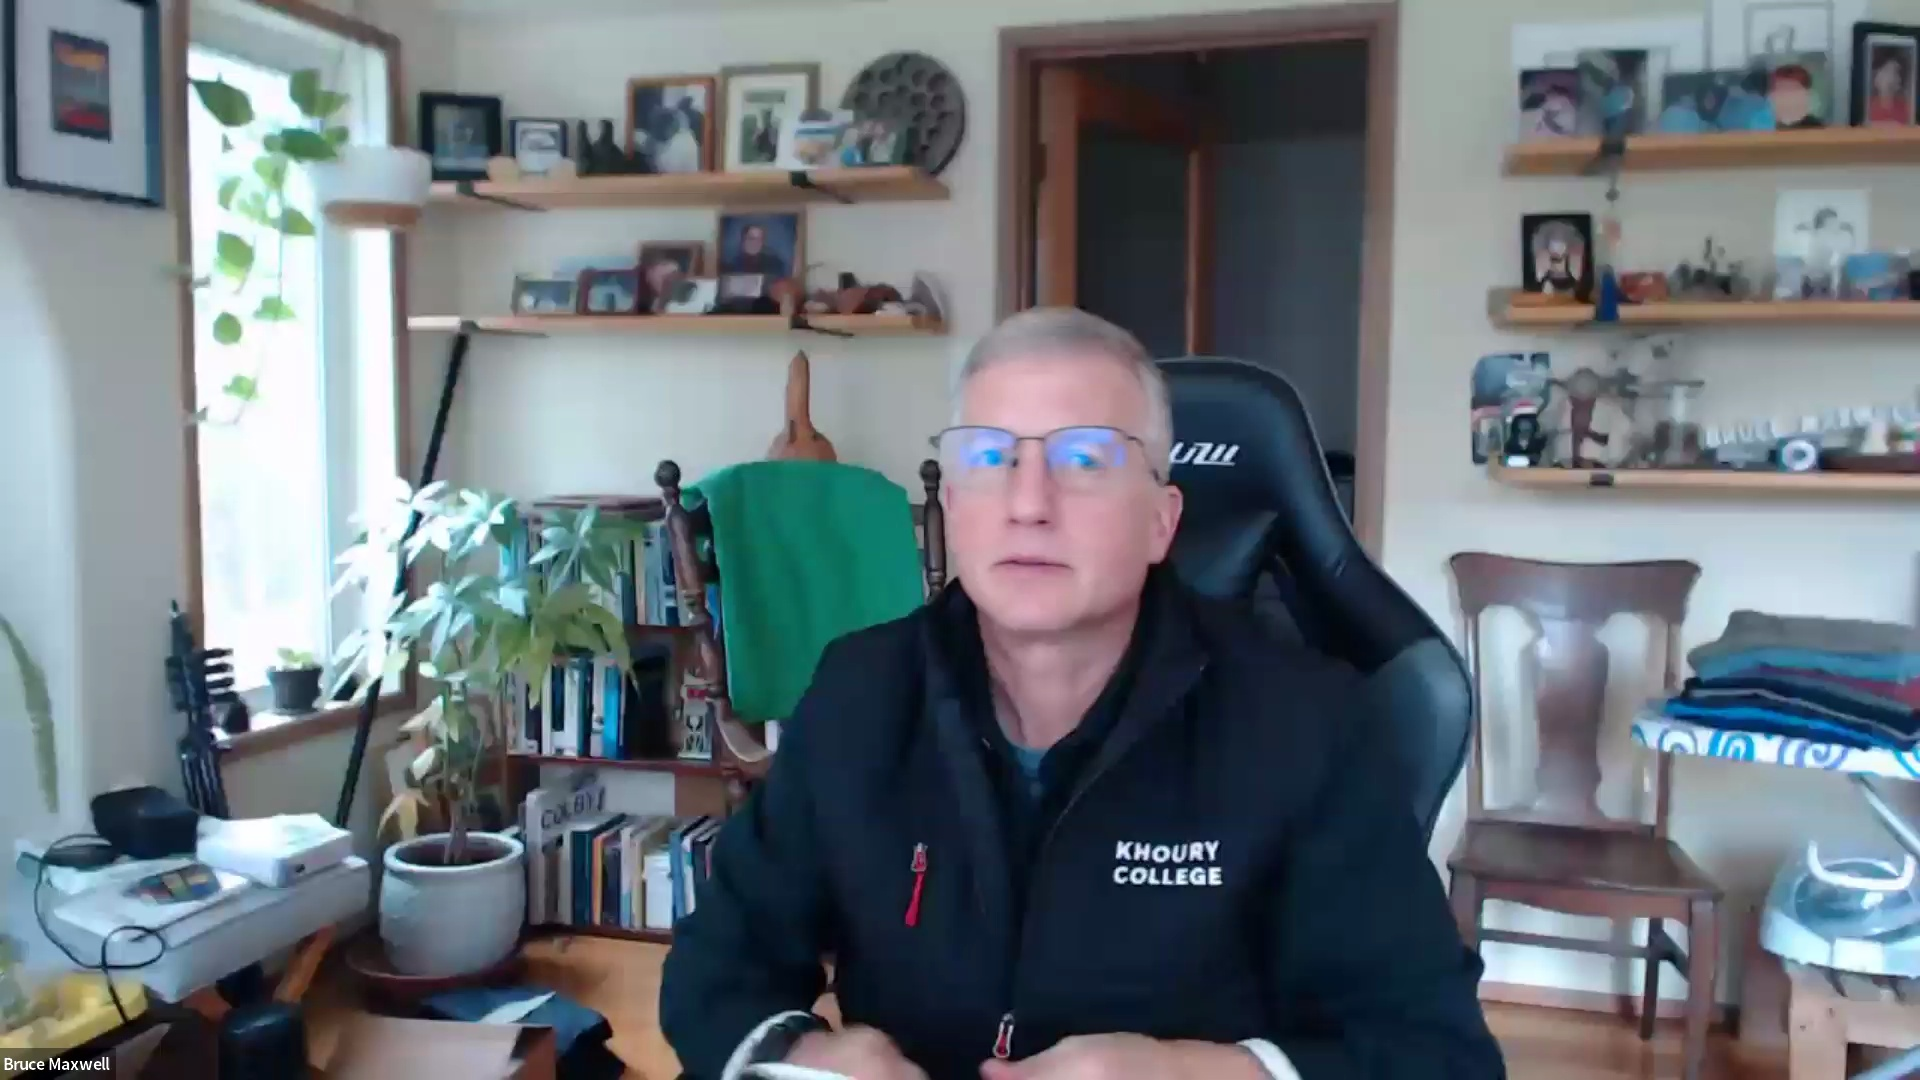
\includegraphics[width=\linewidth]{0000110.jpg}\\{\tiny Frontal, silent}
      \end{minipage}\hfill
      \begin{minipage}{0.47\textwidth}\centering
        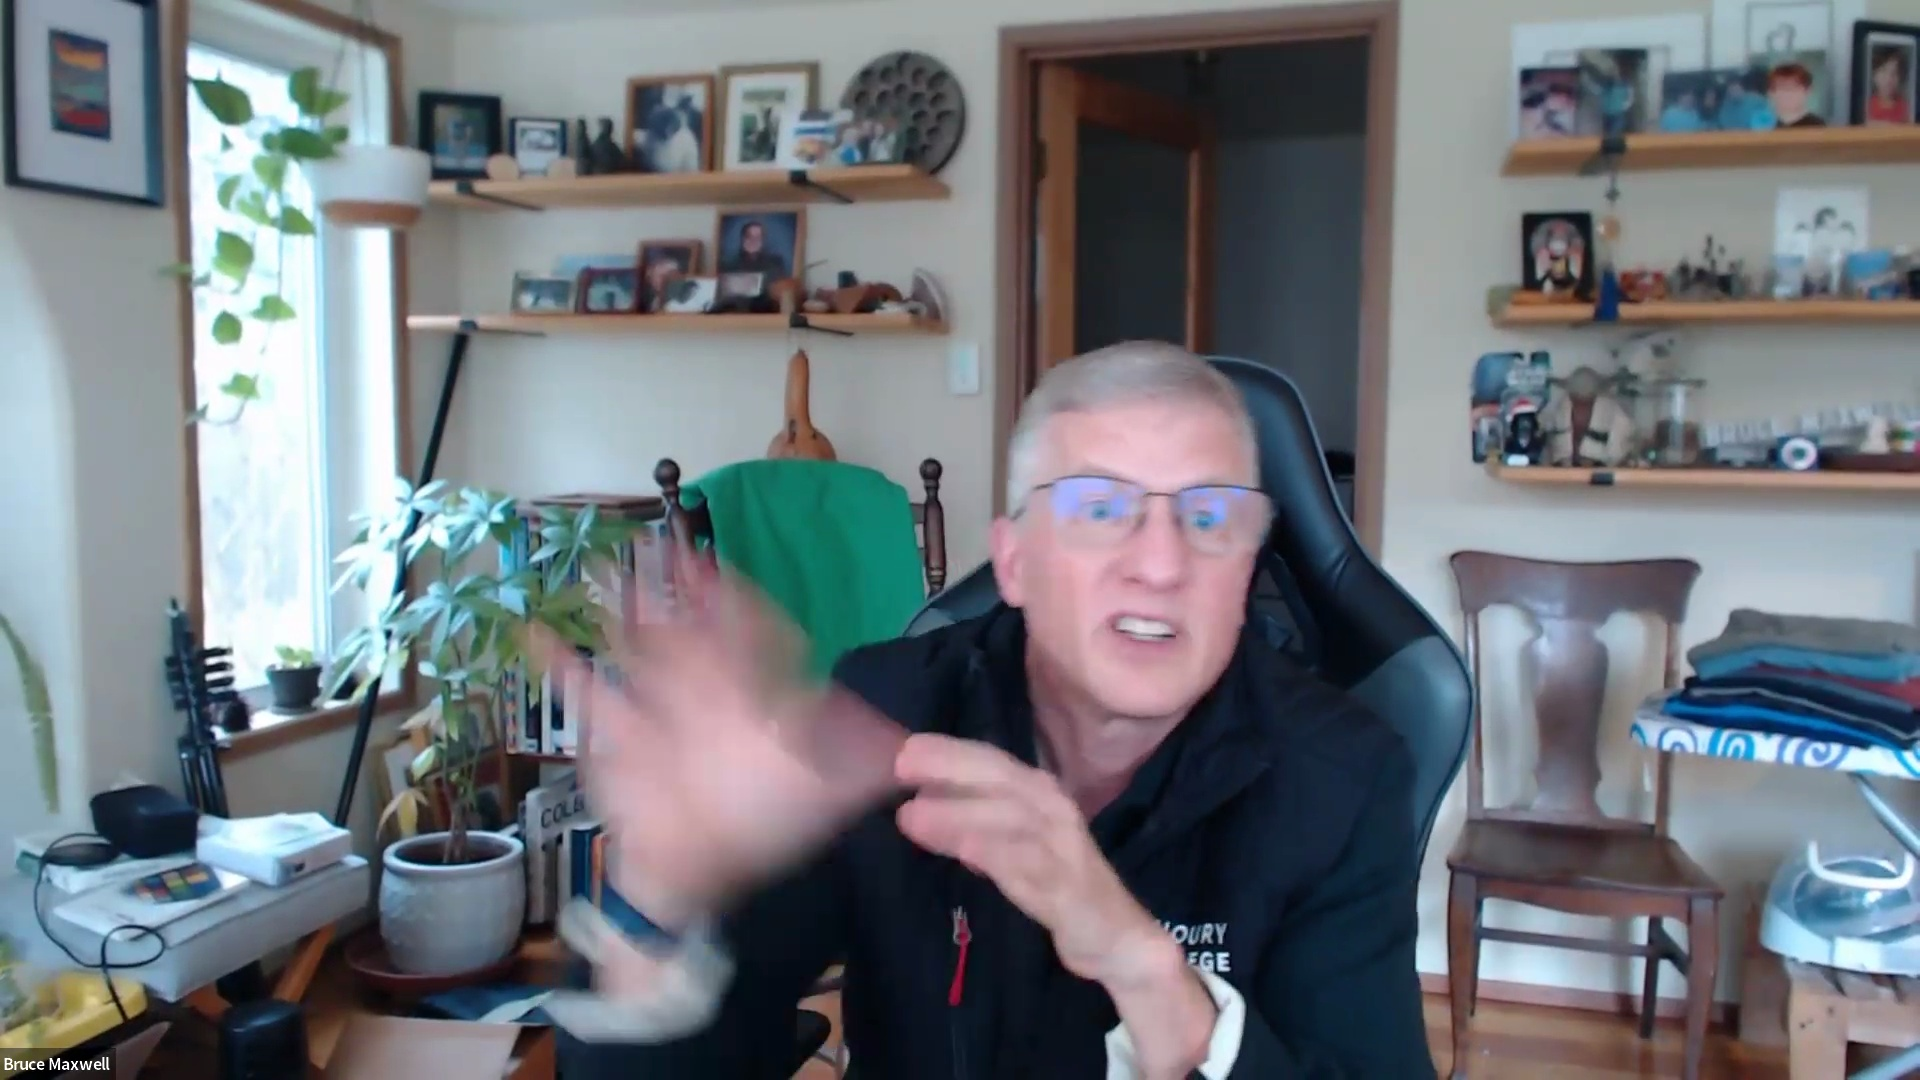
\includegraphics[width=\linewidth]{0014750.jpg}\\{\tiny Speaking + motion blur}
      \end{minipage}\\[4pt]
      \begin{minipage}{0.47\textwidth}\centering
        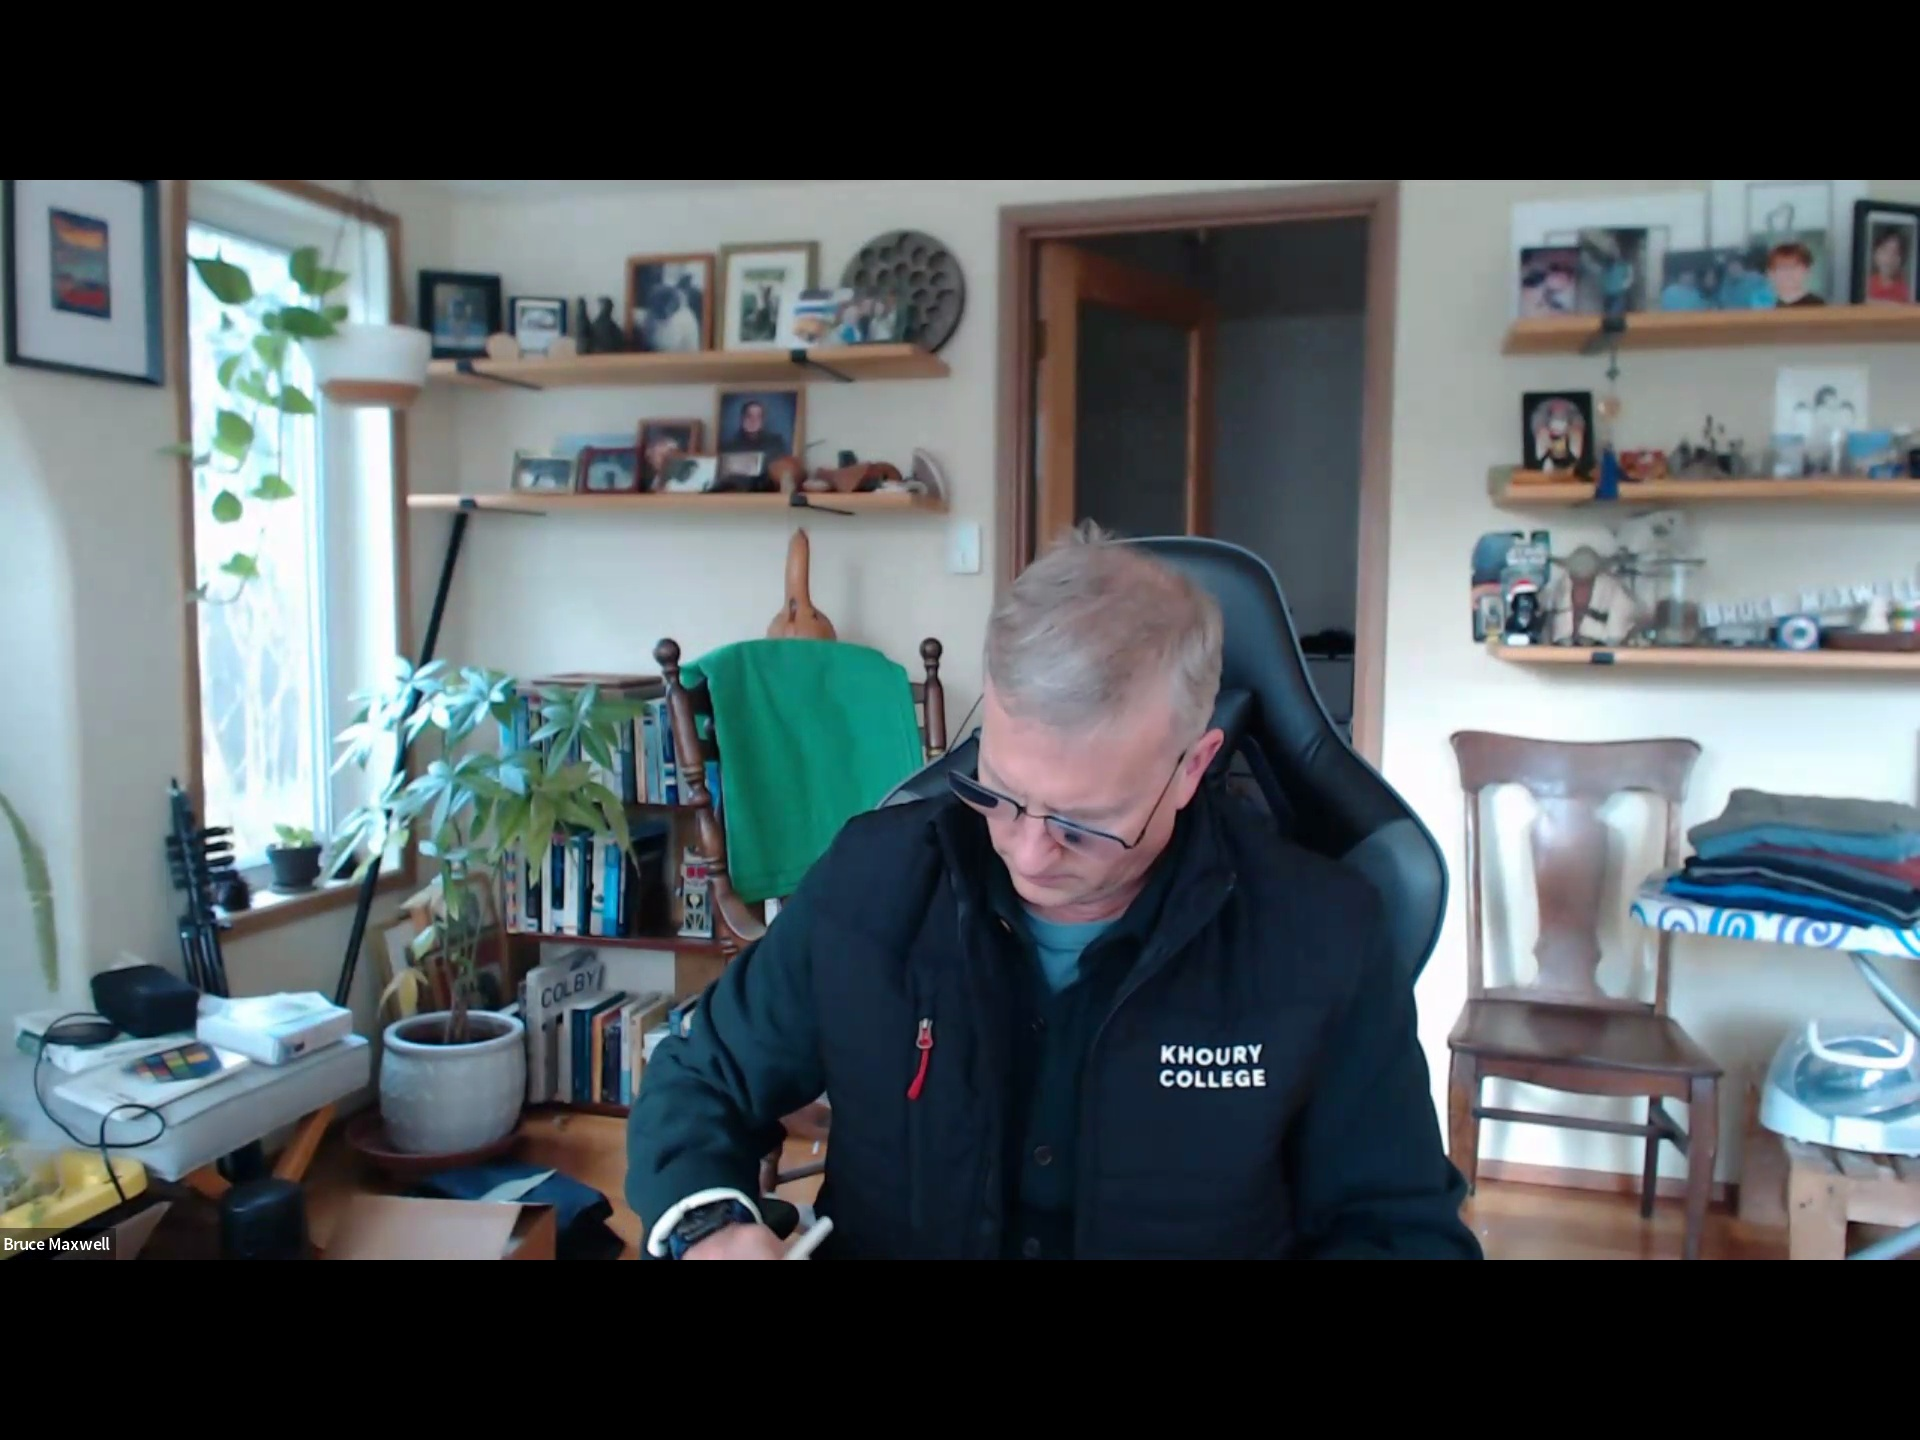
\includegraphics[width=\linewidth]{0000890.jpg}\\{\tiny Head down}
      \end{minipage}\hfill
      \begin{minipage}{0.47\textwidth}\centering
        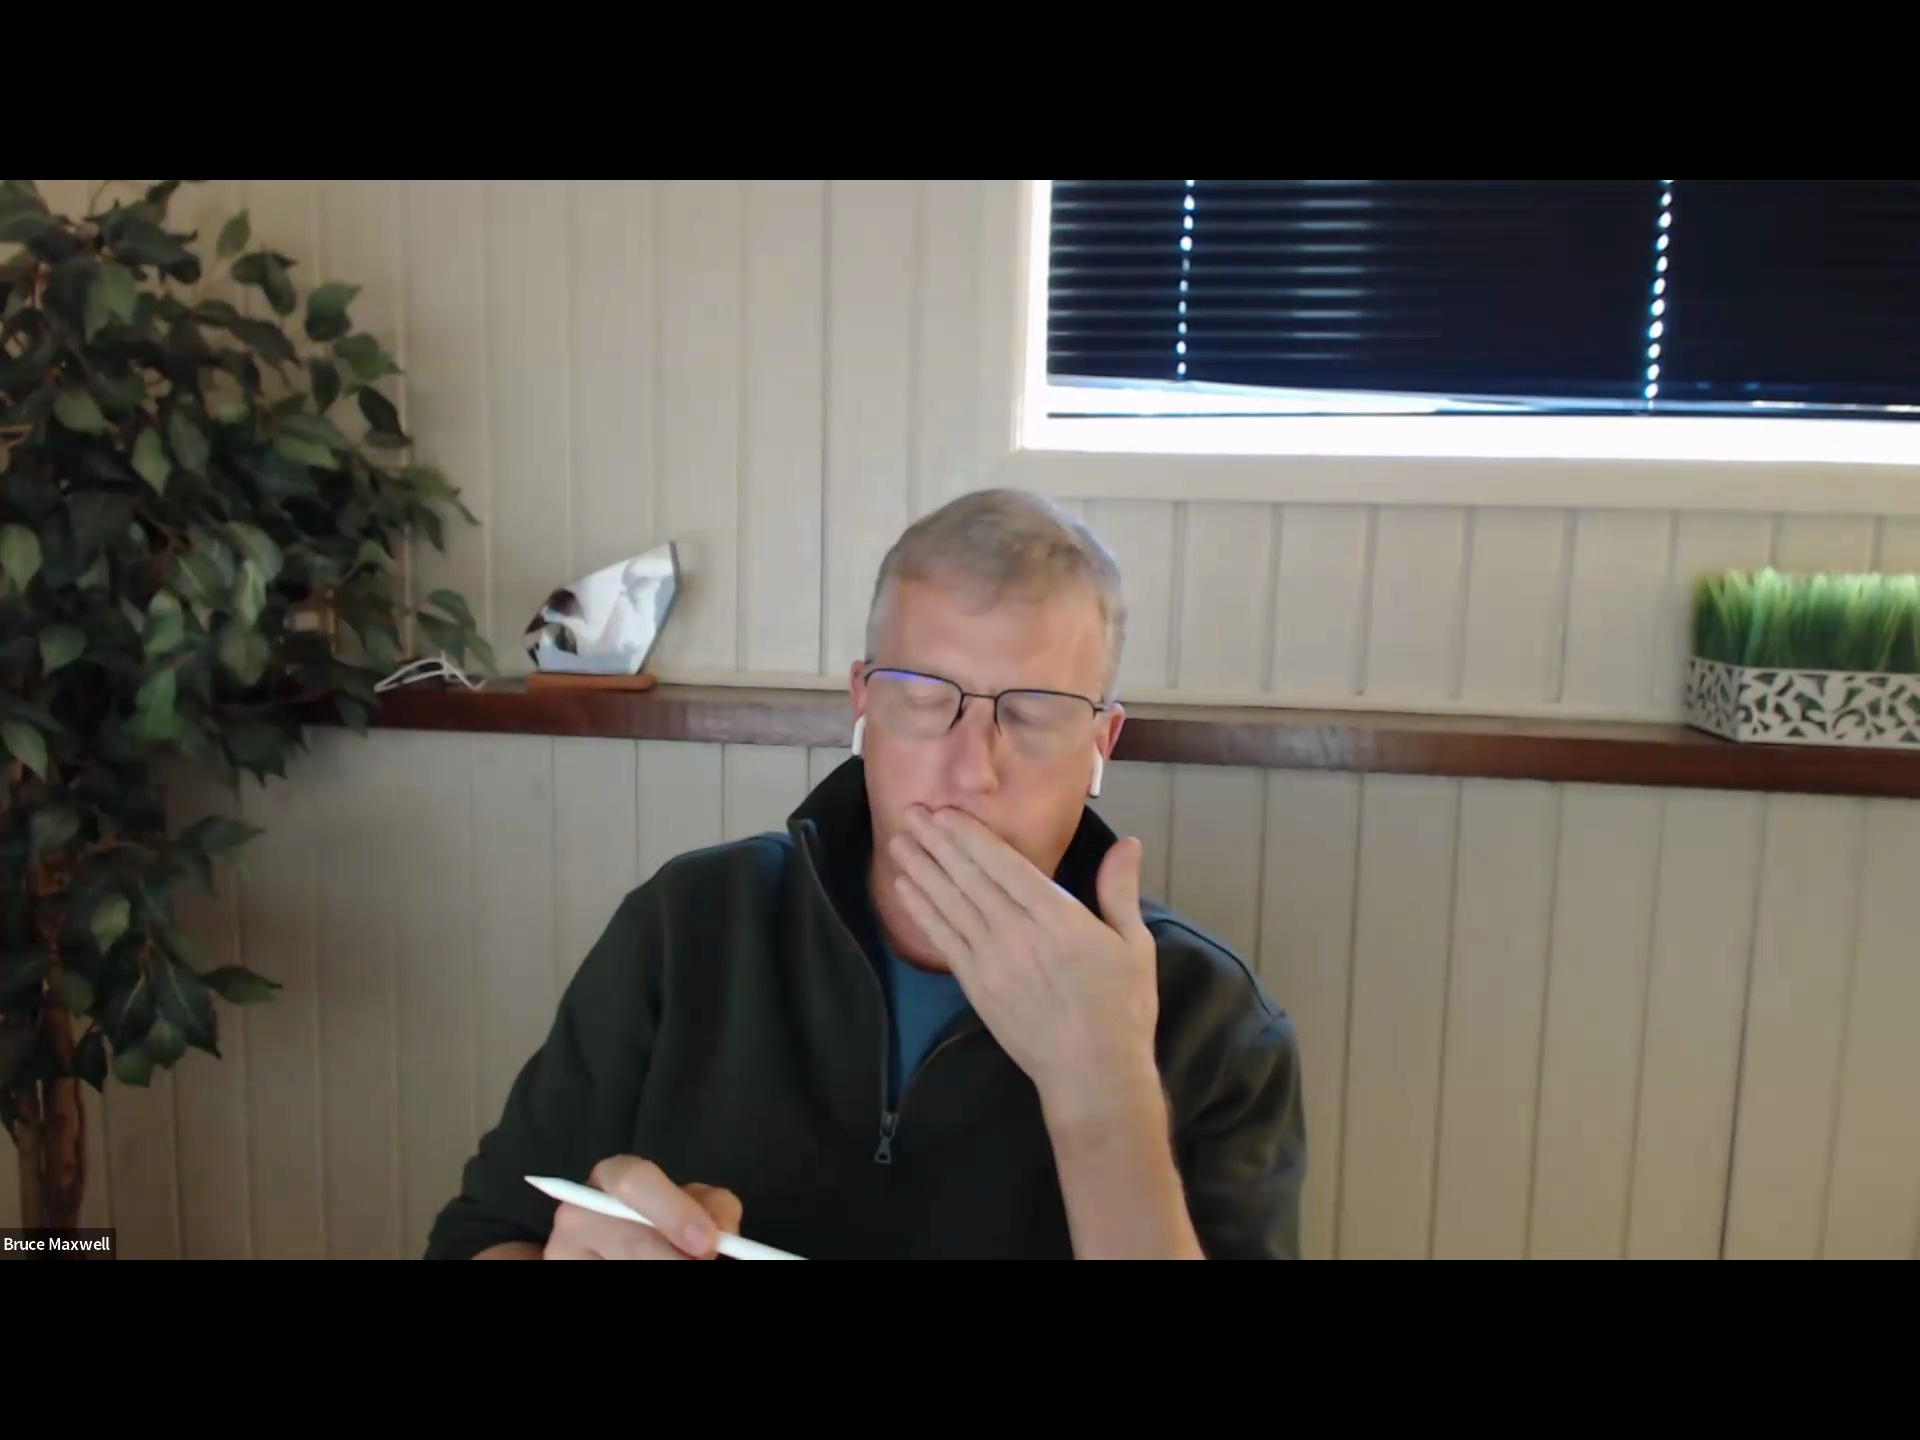
\includegraphics[width=\linewidth]{0000160.jpg}\\{\tiny Hand covering mouth}
      \end{minipage}
    \end{column}
  \end{columns}

  \note{
    \textbf{Context:} This is a frame-level binary classification problem:
    speaking (1) or silent (0). The real challenge is that the model is
    trained on one recording and has to work on all the others — each of
    which has different lighting, pose habits, and scene setup.\\[4pt]
    \textbf{Say:}
    \begin{itemize}
      \item ``For each frame in a video, I want to know: is this person
            currently talking?''
      \item Point to each photo: ``Clean frontal shot. Active speech with
            motion. Head down writing on something. Hand blocking the mouth.''
      \item ``In a real lecture, all of these happen. The question is which
            measurement of the face stays useful despite all of this.''
      \item ``Existing work mostly uses deep learning or audio — I wanted
            to understand which specific visual feature is doing the work.''
    \end{itemize}
  }
\end{frame}

% ═══════════════════════════════════════════════════════════════════════════
% SLIDE 3 — Related Work
% ═══════════════════════════════════════════════════════════════════════════
\begin{frame}{Related Work}

  \begin{block}{Lip reading \& talking-face detection}
    \small\textbf{Chung \& Zisserman (2016, 2017)} trained deep networks
    on lip-region video crops. High accuracy, but the model is a black box:
    no insight into \emph{which} face geometry matters.
  \end{block}

  \begin{block}{Active speaker detection}
    \small\textbf{Roth et al.\ (AVA-ActiveSpeaker, 2020)} who is speaking
    in a multi-person scene? Audio-visual fusion works best, but mouth-region
    cues are consistently the strongest visual signal.
  \end{block}

  \begin{block}{Face landmark detection (our backbone)}
    \small\textbf{Kartynnik et al.\ (MediaPipe Face Mesh, 2019)} detects
    468 face landmarks in real time on a regular CPU. We use this as our
    feature extractor.
  \end{block}

  % \begin{center}
  %   \textit{Our angle: understand \emph{which} features matter, not just maximize accuracy.}
  % \end{center}

  \note{
    \textbf{Context:} These three papers cover the main threads of prior work.
    Chung \& Zisserman showed visual lip motion carries strong speech signal
    but used end-to-end deep networks. Roth et al.'s AVA-ActiveSpeaker is a
    large benchmark (used at Google I/O) for detecting active speakers in
    multi-person video. MediaPipe is Google's open-source face landmarking
    model — it outputs 468 3D point coordinates for any detected face.\\[4pt]
    \textbf{Say:}
    \begin{itemize}
      \item ``Earlier work shows that lip motion is the key visual cue, but
            it uses black-box deep networks. I can't tell from those which
            specific geometric property is driving the result.''
      \item ``MediaPipe gives me exact measurements — like how far apart
            two lip points are — which I can then test individually.''
      \item ``My contribution is replacing the black box with interpretable
            features and testing each one.''
    \end{itemize}
  }
\end{frame}

% ═══════════════════════════════════════════════════════════════════════════
% SLIDE 4 — Methods
% ═══════════════════════════════════════════════════════════════════════════
\begin{frame}{Methods \& Pipeline}

  \begin{columns}[T]
    \begin{column}{0.45\textwidth}
      \head{Pipeline:}

      \vspace{0.2em}
      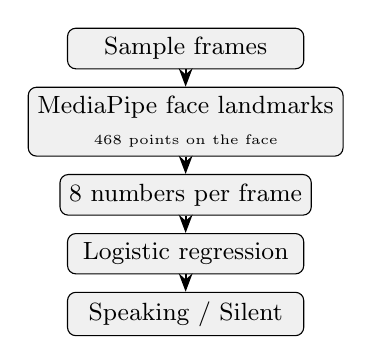
\begin{tikzpicture}[
        box/.style={draw, rounded corners=3pt, fill=gray!12,
                    minimum width=3.0cm, minimum height=0.5cm,
                    font=\small, align=center},
        arr/.style={-Stealth, thick}
      ]
        \node[box] (vid)  {Sample frames};
        \node[box] (mp)   [below=0.22cm of vid]  {MediaPipe face landmarks\\{\tiny 468 points on the face}};
        \node[box] (feat) [below=0.22cm of mp]   {8 numbers per frame};
        \node[box] (clf)  [below=0.22cm of feat] {Logistic regression};
        \node[box] (out)  [below=0.22cm of clf]  {Speaking / Silent};
        \draw[arr] (vid)--(mp);
        \draw[arr] (mp)--(feat);
        \draw[arr] (feat)--(clf);
        \draw[arr] (clf)--(out);
      \end{tikzpicture}

      \vspace{0.3em}
      \head{Train on 1 video. Test on all others.}\\
      {\small No retraining at test time.}
    \end{column}

    \begin{column}{0.52\textwidth}
      \head{8 features computed per frame:}

      \vspace{0.2em}
      % {\small
      % \begin{tabular}{lp{4.2cm}}
      %   \toprule
      %   \textbf{Feature} & \textbf{What it measures} \\
      %   \midrule
      %   Mouth openness & How wide is the mouth open? \\
      %   Eye openness   & How open are the eyes? \\
      %   Yaw, Pitch     & Head angle (left-right, up-down) \\
      %   Motion mean/var & How much did the image move? \\
      %   Brightness     & How bright is the scene? \\
      %   Landmark score & Did the face detector succeed? \\
      %   \bottomrule
      % \end{tabular}}
      \begin{enumerate}
        \item Mouth openness
        \item Eye openness
        \item Yaw
        \item Pitch
        \item Motion mean
        \item Motion var
        \item Brightness
        \item Landmark score
      \end{enumerate}

      % \vspace{0.2em}
      % {\scriptsize\textit{Conditions used to group test results:}
      % Frontal ($<$15° yaw) vs.\ angled.
      % Low vs.\ high motion (split at training median).}
    \end{column}
  \end{columns}

  \note{
    \textbf{Context:} MediaPipe returns 2D/3D coordinates for 468 face
    landmarks. From those, 8 scalar features are derived per frame.
    Mouth openness = Euclidean distance between inner upper and lower lip
    points, divided by frame height for scale invariance. Yaw/pitch are
    estimated via the Perspective-n-Point (PnP) algorithm using 6 landmarks
    with known 3D positions (nose, chin, eye corners, mouth corners).
    Logistic regression with balanced class weights handles class imbalance.\\[4pt]
    \textbf{Say:}
    \begin{itemize}
      \item Walk through the pipeline top to bottom.
      \item ``MediaPipe finds 468 points on the face. I pick 8 simple
            measurements from those — things like how open the mouth is,
            what angle the head is at, how bright the room is.''
      \item ``Then I train a logistic regression classifier — basically a
            weighted combination of those 8 numbers — on one video from
            January, and apply it to all the others without changing anything.''
      \item ``The conditions at the bottom let me compare performance when
            the head is facing the camera vs.\ turned away.''
    \end{itemize}
  }
\end{frame}

% ═══════════════════════════════════════════════════════════════════════════
% SLIDE 5 — Data & Experiments
% ═══════════════════════════════════════════════════════════════════════════
\begin{frame}{Data \& Experiments}

  \begin{columns}[T]
    \begin{column}{0.44\textwidth}
      \head{Dataset:}
      \begin{itemize}\footnotesize
        \item 30 webcam lectures, one subject%, fixed camera
        \item \textbf{Train:} January 45 min recording %(45 min, 1{,}179 frames)
        \item \textbf{Test:} 20 recordings across the full semester
        \item \textbf{Labels:} speaking / silent, hand-annotated %per frame
      \end{itemize}

      \head{Three experiments:}
      \begin{enumerate}\footnotesize
        % \item \textbf{Ablation}: which features matter? %(5-fold CV)
        % \item \textbf{Generalization}: how well does it transfer to new recordings?
        % \item \textbf{Fine-tuning}: does adding a few labeled frames from the
        %       test video help?
        \item Ablation
        \item Generalization
        \item Fine-tuning
      \end{enumerate}
    \end{column}

    \begin{column}{0.53\textwidth}
      \begin{figure}
        \centering
        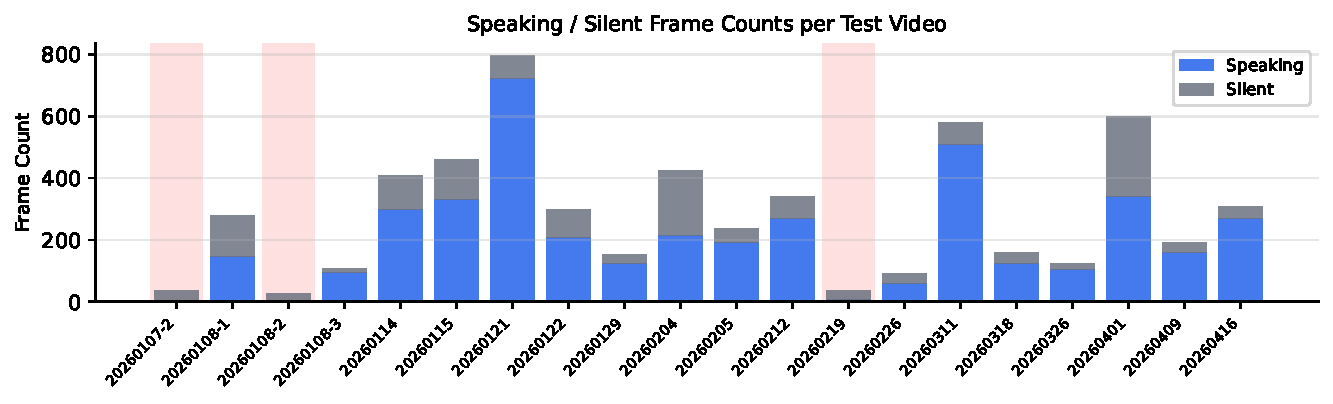
\includegraphics[width=\linewidth, height=2.6cm, keepaspectratio]{class_balance.pdf}
        \caption*{\scriptsize Speaking vs.\ silent frame counts per recording}
      \end{figure}
    \end{column}
  \end{columns}

  \note{
    \textbf{Context:} All recordings are of the presenter (you). The
    train/test split is strictly by video — no frames from test videos
    appear during training. This prevents data leakage and makes the
    evaluation honest. Labels were created manually using a custom
    scrubbing tool: step through each sampled frame and press a key
    for speaking or silent. F1 score (not accuracy) is the main metric
    because class balance varies a lot across recordings.\\[4pt]
    \textbf{Say:}
    \begin{itemize}
      \item ``30 lectures across one semester, all me, same webcam.
            Trained on one from January, tested on everything else.''
      \item ``I manually labeled about 7,000 frames total — stepping
            through each video frame by frame.''
      \item ``The bar chart shows the speaking/silent split per recording.
            The red-highlighted ones had almost no speaking frames at all,
            so I excluded them from the aggregate numbers.''
      \item ``Three experiments: which features matter, how well it
            transfers, and whether adding a few labels from the test
            video fixes failures.''
    \end{itemize}
  }
\end{frame}

% ═══════════════════════════════════════════════════════════════════════════
% SLIDE 6 — Ablation Results
% ═══════════════════════════════════════════════════════════════════════════
\begin{frame}{Experiment 1: Which Feature Actually Matters?}

  \begin{columns}[T]
    \begin{column}{0.54\textwidth}
      \begin{figure}
        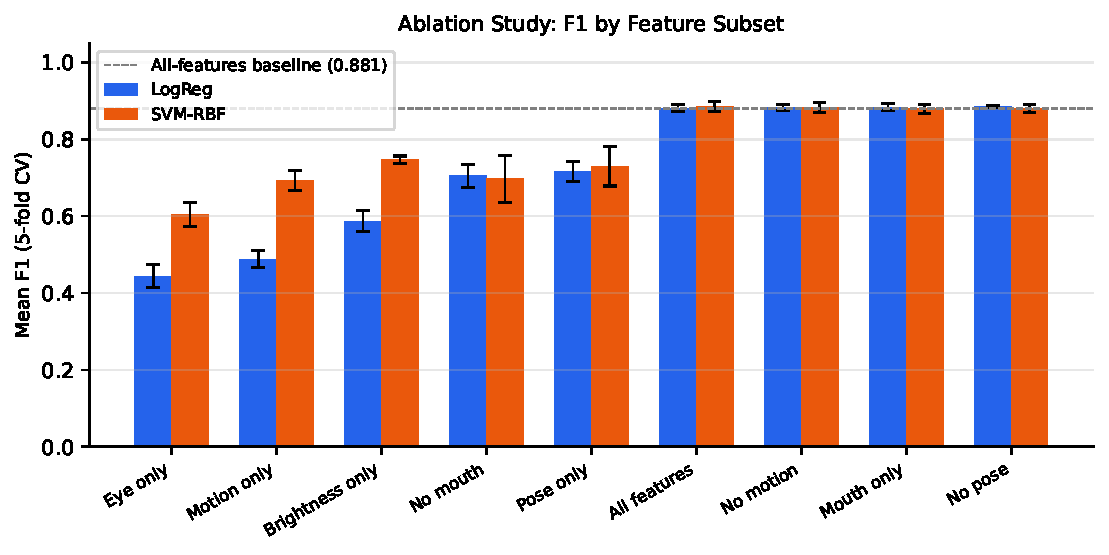
\includegraphics[width=\linewidth, height=5.2cm, keepaspectratio]{ablation.pdf}
        \caption*{\scriptsize F1 score per feature group}
      \end{figure}
    \end{column}

    \begin{column}{0.43\textwidth}
      \vspace{0.4em}
      \head{F1 scores (logistic regression):}
      \vspace{0.3em}

      \begin{tabular}{lc}
        \toprule
        \textbf{Feature set} & \textbf{F1} \\
        \midrule
        Eye only            & 0.444 \\
        Motion only         & 0.488 \\
        Brightness only     & 0.587 \\
        Pose only           & 0.717 \\
        \midrule
        All 8 features      & 0.881 \\
        Everything but mouth & 0.705 \\
        \alert{\textbf{Mouth only}} & \alert{\textbf{0.883}} \\
        \bottomrule
      \end{tabular}

      \vspace{0.5em}
      % \alert{\textbf{Finding 1:}} Mouth openness alone\\
      % matches all 8 features combined.\\[0.3em]
      % {\small Remove it $\to$ $-18$ point drop.\\
      % Add anything else $\to$ no gain.}
    \end{column}
  \end{columns}

  \note{
    \textbf{Context:} An ablation study systematically tests feature
    subsets to isolate which ones carry signal. 5-fold cross-validation
    on the training video (January) gives an honest within-distribution
    estimate. F1 = harmonic mean of precision and recall — better than
    accuracy when classes are imbalanced. The ``no mouth'' row uses all
    7 other features; it's worse than mouth alone.\\[4pt]
    \textbf{Say:}
    \begin{itemize}
      \item ``I tested every feature in isolation and in combinations.
            The result is pretty striking.''
      \item ``Mouth openness alone — just how far apart two lip points
            are — gets F1 of 0.883. The full 8-feature model gets 0.881.
            They're essentially the same.''
      \item Point to the ``Everything but mouth'' row: ``If I remove
            just the mouth and keep everything else, it drops to 0.705.
            That's an 18-point swing.''
      \item ``So mouth openness is both necessary and sufficient.
            All the other features add nothing.''
      \item ``This makes intuitive sense: most speech sounds require the
            jaw to open. It's a direct physical signal.''
    \end{itemize}
  }
\end{frame}

% ═══════════════════════════════════════════════════════════════════════════
% SLIDE 7 — Generalization + Fine-Tuning
% ═══════════════════════════════════════════════════════════════════════════
\begin{frame}{Experiments 2 \& 3: Does It Generalize?}

  \begin{columns}[T]
    \begin{column}{0.55\textwidth}
      \begin{figure}
        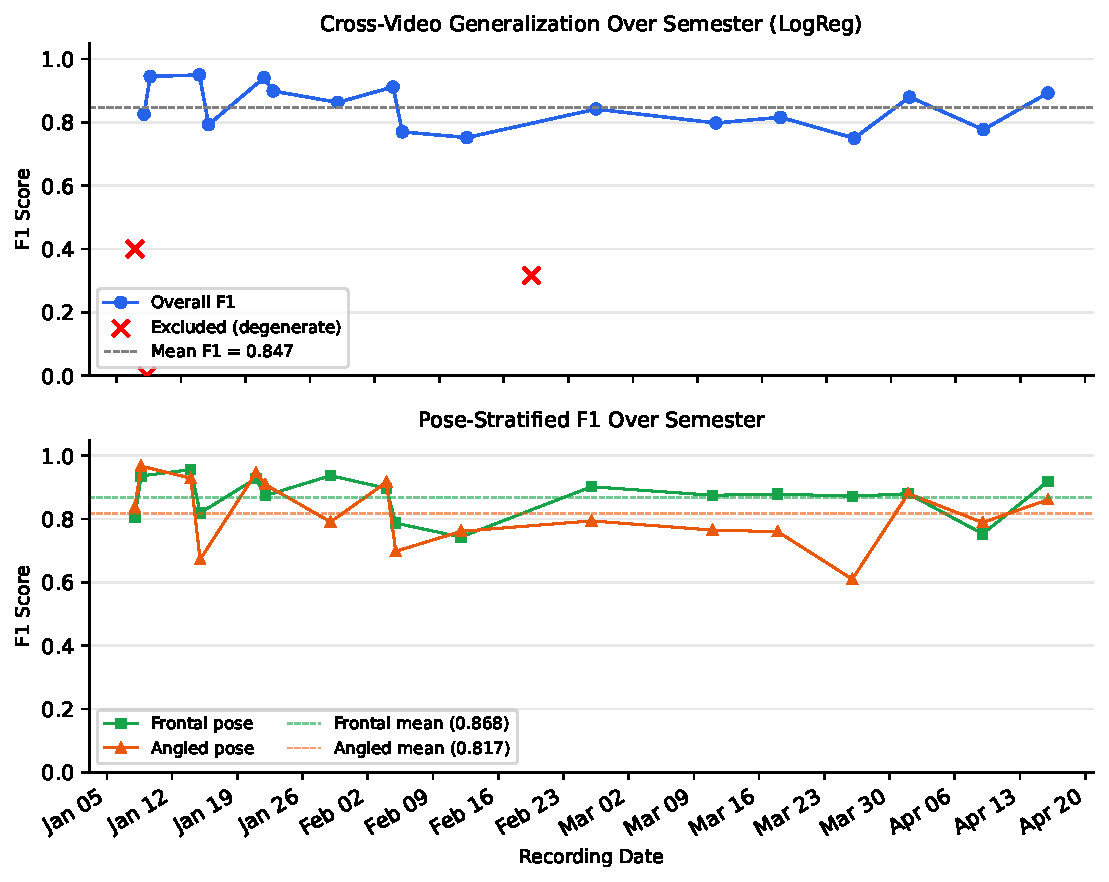
\includegraphics[width=\linewidth, height=5cm, keepaspectratio]{generalization.pdf}
        \caption*{\scriptsize F1 per recording across the semester (top).
          Head-facing-camera vs.\ head-turned F1 (bottom).}
      \end{figure}
    \end{column}

    \begin{column}{0.42\textwidth}
      \vspace{0.4em}

      {\footnotesize
      \textbf{Performance:}
      \begin{itemize}
        \item \textbf{Mean F1 = 0.848}, %no retraining (range 0.75–0.95)
        \item Frontal: 0.869 / Turned: 0.817
        \item Big drops = head \emph{down} %(mouth out of frame)
      \end{itemize}
      %\alert{\textbf{Finding 2:}} Generalizes well across the semester.

      \smallskip
      \textbf{Adding labeled frames from test video:}
      \begin{itemize}
        \item 25, 50, 100 frames tried on 5 videos
        \item 1 improved; rest flat or worse
      \end{itemize}
      %\alert{\textbf{Finding 3:}} Fine-tuning doesn't consistently help.
      }
    \end{column}
  \end{columns}

  \note{
    \textbf{Context:} The model trained on January is applied directly to
    each of the other 20 recordings with no changes. Frontal vs.\ angled
    is defined by yaw angle: $<$15° is frontal, $\geq$15° is angled.
    Three recordings are excluded: two had almost no speaking frames
    (so F1 is undefined), one had the head pointed down for extended
    periods so the mouth was off-screen. Fine-tuning merges n labeled
    frames from the target video back into training and retrains.\\[4pt]
    \textbf{Say:}
    \begin{itemize}
      \item ``Trained once in January, tested across the whole semester
            without touching the model. Mean F1 of 0.848 — pretty strong.''
      \item Point to the top plot: ``Most recordings land above 0.80.
            The three red crosses are excluded outliers.''
      \item ``The frontal vs.\ turned-head gap is small on average.
            The big drops in specific recordings come from the head
            pointing \emph{down} — so the mouth is out of frame entirely.
            That's a different problem from ordinary yaw variation.''
      \item ``I also tried adding a small number of labeled frames from
            each test video to see if that helps. For 4 out of 5 videos,
            it didn't. The mouth feature already works across recordings.''
    \end{itemize}
  }
\end{frame}

% ═══════════════════════════════════════════════════════════════════════════
% SLIDE 8 — Summary & Takeaways
% ═══════════════════════════════════════════════════════════════════════════
\begin{frame}{Summary \& Takeaways}

  \begin{columns}[T]
    \begin{column}{0.54\textwidth}
      \head{Three findings:}
      \begin{enumerate}\footnotesize
        % \item \textbf{Mouth openness is all you need.}
        %       One measurement matches the full model (F1\,$\approx$\,0.88).
        % \item \textbf{It transfers across the semester.}
        %       Mean F1 = 0.848 on 17 test recordings with no retraining.
        %       Failures = mouth occluded, not ordinary pose variation.
        % \item \textbf{Fine-tuning doesn't help.}
        %       Adding labeled frames from test videos: no consistent gain.
        \item Mouth openness is all you need
        \item Generalization across semester
        \item Fine-tuning doesn't help
      \end{enumerate}

      \vspace{0.15em}
      \head{Limitations:}
      \begin{itemize}\footnotesize
        \item Single subject %— findings are for one speaker only
        \item One frame at a time %— no temporal smoothing
        \item Fails when the mouth is physically hidden
      \end{itemize}
    \end{column}

    \begin{column}{0.43\textwidth}
      \head{What I learned:}
      \begin{itemize}\footnotesize
        % \item \textbf{Ablate before you model.} The answer was one
        %       geometric measurement — no neural network needed.
        % \item \textbf{Use F1, not accuracy.} Class imbalance is real;
        %       accuracy hides it.
        % \item \textbf{Outliers are the interesting part.} Understanding
        %       \emph{why} 3 recordings failed taught me more than the
        %       17 that worked.
        % \item \textbf{Simple pipelines are underrated.} Laptop-scale
        %       CPU, 30 videos, meaningful conclusions.
        \item Use F1 over accuracy
        \item Outliers are the interesting part
        \item Simple pipelines are underrated
      \end{itemize}

      \vspace{0.1em}
      \head{Future directions:}
      \begin{itemize}\footnotesize
        \item Smoothing to reduce frame-level jitter
        \item Test across multiple speakers
        \item Add audio for occlusion robustness
      \end{itemize}
    \end{column}
  \end{columns}

  \note{
    \textbf{Context:} Three experiments map directly to three findings.
    The headline result is surprising in its simplicity: one normalized
    distance between two lip landmarks beats every other feature and
    every combination.\\[4pt]
    \textbf{Say:}
    \begin{itemize}
      \item Recap each finding in one sentence each.
      \item ``The big surprise was Finding 1 — I expected the full model
            to win, but a single lip distance matched it exactly.''
      \item Pivot to the right column: ``What I took away from this
            project is that ablation — systematically testing what you
            actually need — should come before picking a model.''
      \item ``F1 over accuracy: several of my recordings had 80\% silence.
            A dumb classifier that always predicts silent would look
            great by accuracy. F1 catches that.''
      \item Close: ``Happy to take questions.''
    \end{itemize}
  }
\end{frame}

\end{document}
